\chapter{Relatividad especial: sistemas de referencia, simultaneidad y transformación de Lorentz}

La relatividad es el principio según el cual las leyes de la física no dependen del sistema inercial que usemos para describirlas. Nuestra primera tarea es la cinemática: el significado del espacio, el tiempo, el movimiento, la sincronización y la transformación de un sistema inercial a otro. Después viene la dinámica, con la energía, el momento lineal y la fuerza relativistas, el análogo de la ecuación del movimiento de Newton y el significado de \(E=mc^2\). Cuando hayamos asentado bien esa estructura, podremos abordar conceptualmente la relatividad general mediante el espaciotiempo curvo, el movimiento de partículas en un campo gravitatorio dado, los agujeros negros y la expansión del universo, sin empezar por el difícil problema de resolver las ecuaciones de campo de Einstein.

Conviene distinguir entre rigor conceptual y rigor matemático. No usaremos ninguna aproximación que sepamos falsa. En cambio, pondremos el énfasis en los efectos de un campo gravitatorio sobre los relojes, las partículas y la geometría, y dejaremos para más adelante el formalismo necesario para construir soluciones arbitrarias de las ecuaciones de campo. La relatividad especial requiere un tratamiento más explícito, porque todo el razonamiento posterior se apoya en su cinemática.

Por tanto, lo adecuado es empezar no con una fórmula célebre, sino con una descripción precisa de lo que un observador entiende por lugar y tiempo.

\section{Un sistema de referencia es un sistema de coordenadas físico}

Imaginemos el espacio lleno de una retícula arbitrariamente fina de reglas de un metro. Cada punto de la retícula está etiquetado con tres coordenadas espaciales y, en cada punto, hay un reloj. En conjunto, las reglas y los relojes constituyen un sistema de referencia.

\begin{definition}Un \emph{suceso} es algo que ocurre en un lugar y en un instante. En una dimensión espacial, sus coordenadas se escriben \((x,t)\); en tres dimensiones, son \((x,y,z,t)\).\end{definition}

La física newtoniana añade una hipótesis potente: todos los relojes ideales pueden sincronizarse de una vez y para siempre. El tiempo es universal. Se puede desplazar un reloj y un observador puede llevar un reloj de pulsera, pero se supone que todos están de acuerdo en el mismo \(t\) en todas partes. A esto a veces se lo llama tiempo absoluto; podemos imaginarlo como el tiempo de Dios, un único reloj para todo el mundo.

El principio de relatividad es anterior a Einstein. Su imagen natural es la de un tren que se mueve uniformemente por raíles perfectamente lisos, sin traqueteos ni sacudidas. Dentro del tren podemos lanzar y atrapar pelotas exactamente igual que en un tren detenido en la estación. Hacer malabarismos es un experimento de mecánica sorprendentemente completo: requiere medir el tiempo, tener en cuenta la gravedad y la alineación, y controlar repetidamente las trayectorias. Si el tren se mueve a velocidad constante, ninguna de esas reglas cambia. Una pelota lanzada verticalmente vuelve a la misma mano; el tren no se desliza por debajo. Galileo reconoció este hecho y Newton lo expresó sistemáticamente en sus leyes del movimiento.

Antes de Galileo, resultaba tentador pensar que el tren en movimiento avanzaría mientras la pelota está en el aire y que quien hace malabarismos tendría que estirarse hacia atrás o hacia delante para atraparla. El error consiste en olvidar que la pelota ya comparte la velocidad horizontal del tren cuando sale de la mano. Ningún experimento realizado dentro del vagón que se mueve suavemente revela un estado especial de reposo absoluto. Solo se observa el movimiento relativo entre los dos trenes.

Por tanto, el tren en reposo y el que se mueve uniformemente son dos sistemas inerciales. Antes de Einstein, se relacionaban mediante transformaciones galileanas.

\section{Representación del espaciotiempo}

Por el momento, omitimos \(y\) y \(z\), y representamos el tiempo en vertical y la posición \(x\) en horizontal. Cada punto del dibujo es un suceso. La línea \(x=0\) es la historia, o \emph{línea de universo}, del origen espacial. Las líneas verticales cercanas \(x=1,2,3,\ldots\) son las líneas de universo de los demás puntos de la retícula. Las líneas horizontales son conjuntos de sucesos con un mismo tiempo.

\begin{figure}[H]\centering
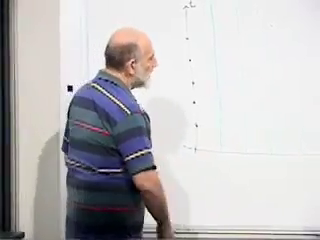
\includegraphics[width=0.62\textwidth]{lecture_01_figure_02.png}\caption{El eje temporal del sistema en reposo y las primeras líneas de universo de la retícula espacial.}\lectureframe{00:16:38}\end{figure}

La misma construcción se aprecia mejor en un dibujo idealizado:

\begin{figure}[H]\centering
\begin{tikzpicture}[scale=0.95]
\draw[->] (-1.2,0) -- (5.2,0) node[right] {$x$};
\draw[->] (0,-0.2) -- (0,4.8) node[above] {$t$};
\foreach \x in {-1,1,2,3,4}
  \draw[gray!65] (\x,0) -- (\x,4.4);
\foreach \y in {1,2,3,4}
  \draw[gray!65] (-1.0,\y) -- (4.4,\y);
\fill (0,0) circle (1.5pt);
\node[below left] at (0,0) {$0$};
\node[left] at (0,1) {$1$};
\node[left] at (0,2) {$2$};
\node[left] at (0,3) {$3$};
\node[below] at (1,0) {$1$};
\node[below] at (2,0) {$2$};
\node[below] at (3,0) {$3$};
\end{tikzpicture}\caption{Una retícula de espaciotiempo en reposo. Las líneas verticales tienen posición constante; las horizontales, tiempo constante.}\end{figure}

La retícula es imaginaria y su espaciado es arbitrario. Podemos usar metros, centímetros, micras o cualquier intervalo aún menor que tenga sentido físico. Su propósito es asignar una coordenada precisa a cada suceso.

La expresión «sistema de referencia» adquiere ahora un contenido operacional. No es simplemente un punto de vista ni una persona que mira en cierta dirección. Es un aparato de coordenadas extendido. Para un suceso dado, las reglas locales especifican dónde ocurrió y el reloj local indica cuándo. Así podemos comparar otras magnitudes físicas entre sistemas de referencia: la posición y la velocidad de una partícula, su energía, quizá la temperatura de un cuerpo y, más adelante, su momento lineal y su fuerza. La comparación más sencilla es la que involucra \(x\) y \(t\), así que empezaremos por ahí.

Coloquemos ahora una segunda retícula en un tren que se mueve en la dirección positiva de \(x\) con velocidad constante \(v\). Hagamos coincidir los orígenes en \(t=0\). Entonces, el origen móvil sigue la trayectoria
\begin{equation}
x=vt.
\end{equation}
Cada uno de los demás puntos fijos del tren sigue una línea de universo paralela e inclinada. Esa inclinación expresa geométricamente que el tren cambia de posición con el paso del tiempo.

Supongamos que el punto trasero del tren es el origen primado. En \(t=0\) coincide con el origen de la estación. En un tiempo posterior \(t\), su coordenada en reposo es \(vt\). Así pues, un suceso cercano de coordenada \(x\) está a solo \(x-vt\) del origen del tren. Por eso la transformación implica una resta y no una regla algebraica arbitraria.

Sean \((x,t)\) las coordenadas de un suceso en el sistema de referencia de la estación y \((x',t')\) sus coordenadas en el del tren. Galileo y Newton mantienen el tiempo universal:
\begin{equation}
t'=t.
\end{equation}
Durante el intervalo \(t\), el origen móvil avanza \(vt\), así que la distancia entre ese origen y el suceso es
\begin{equation}
x'=x-vt.
\end{equation}
En conjunto:
\begin{align}
t'&=t, & x'&=x-vt.
\label{eq:galilean-forward}
\end{align}
Al despejar las coordenadas no primadas, obtenemos la transformación inversa:
\begin{align}
t&=t', & x&=x'+vt'.
\label{eq:galilean-inverse}
\end{align}

\begin{figure}[H]\centering
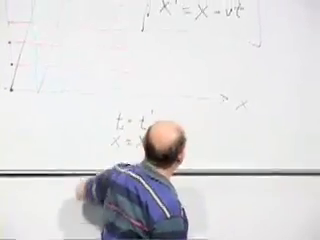
\includegraphics[width=0.72\textwidth]{lecture_01_figure_03.png}\caption{La transformación galileana escrita junto a las dos retículas del espaciotiempo.}\lectureframe{00:21:57}\end{figure}

El primer par indica al observador móvil cómo transformar las coordenadas proporcionadas por el observador en reposo. El par inverso transforma las coordenadas de vuelta. Esta conversión recíproca entre descripciones es el contenido matemático de la relatividad galileana.

La sustitución \(t\to t'\) en la fórmula espacial inversa solo es inocua porque la teoría galileana ya ha establecido que \(t=t'\). Conviene advertir esta hipótesis desde ahora. En la teoría de Einstein, las dos coordenadas temporales serán distintas, y estas sustituciones ya no serán automáticas.

\begin{classroomqa}\audiencequestion{Si se aleja un reloj y luego se lo trae de vuelta, ¿cómo podemos saber que el movimiento no lo aceleró primero y luego lo frenó, ocultando el efecto cuando se comparan los relojes?\lecturetimestamp{00:23:09}}\lecturerresponse{Galileo no podría haber establecido el tiempo universal con la precisión moderna; era una conjetura física. Podemos ponerla a prueba de muchas maneras: llevar buenos relojes en direcciones opuestas, repetir el viaje hacia el norte--sur y también hacia el este--oeste, mover un reloj alrededor del otro o intercambiar señales horarias sin reunir los relojes. A velocidades ordinarias, todas esas pruebas concuerdan con gran precisión. Si los relojes son lo bastante precisos o las velocidades lo bastante altas, aparece una pequeña discrepancia. Que falle la hipótesis del tiempo universal no significa que el experimento tenga un defecto; es uno de los fenómenos que la relatividad especial debe explicar.}\end{classroomqa}

\section{Invariantes galileanos y ley de Newton}

Un invariante es una magnitud en la que coinciden todos los observadores inerciales considerados. Las coordenadas no tienen por qué ser invariantes. Lo que importa es que las leyes formuladas con ellas conserven la misma forma.

El término se usa tanto como sustantivo como adjetivo. Un número puede ser un invariante y una ecuación puede ser invariante bajo una transformación. Distinguir entre magnitudes invariantes y leyes invariantes evita una confusión habitual: la relatividad no afirma que todos los observadores obtengan las mismas coordenadas para todo. Afirma que la ley física que relaciona sus mediciones tiene la misma forma.

Tomemos dos sucesos simultáneos en las posiciones \(x_1\) y \(x_2\). La ecuación~\eqref{eq:galilean-forward} da
\begin{align}
x_1'&=x_1-vt,\\
x_2'&=x_2-vt.
\end{align}
Por tanto, su separación es
\begin{equation}
x_2'-x_1'=(x_2-vt)-(x_1-vt)=x_2-x_1.
\end{equation}
En la física galileana, la distancia entre sucesos que ocurren al mismo tiempo es invariante, aunque las posiciones individuales no lo sean.

\begin{classroomqa}\audiencequestion{¿Las dos apariciones de \(t\) en esa resta se refieren realmente al mismo tiempo?\lecturetimestamp{00:28:16}}\lecturerresponse{Sí. Hemos elegido deliberadamente los dos sucesos \((x_1,t)\) y \((x_2,t)\). Están sobre una misma línea horizontal de tiempo constante. Por tanto, el término común \(vt\) se cancela. Si los sucesos ocurrieran en tiempos distintos, este razonamiento no demostraría que la separación espacial fuera invariante.}\end{classroomqa}

Describamos ahora una partícula mediante una trayectoria \(x(t)\). El observador del tren le asigna
\begin{equation}
x'(t)=x(t)-vt.
\end{equation}
Al derivar una vez, obtenemos la conocida regla de suma de velocidades:
\begin{equation}
\frac{dx'}{dt}=\frac{dx}{dt}-v.
\end{equation}
La posición y la velocidad dependen del sistema de referencia. Un observador que se desplaza junto a una flecha la ve moverse más despacio que otro situado junto a la vía.

Derivemos de nuevo. Como la velocidad relativa \(v\) es constante,
\begin{equation}
\frac{d^2x'}{dt^2}=\frac{d^2x}{dt^2}.
\end{equation}
La aceleración es invariante bajo una transformación galileana. Esto sugiere con fuerza por qué la ley de Newton se expresa en términos de aceleración y no de posición o velocidad.

Esta es la aceleración de un objeto observado, no la aceleración del observador del tren. Ambos sistemas son inerciales, así que ninguno acelera respecto del otro. Los objetos pueden acelerarse hacia la izquierda o la derecha en cualquiera de las dos descripciones, y los dos observadores coinciden en el valor de esa aceleración, aunque discrepen sobre la posición y la velocidad del objeto.

Supongamos que dos partículas ejercen una fuerza entre sí y que esta depende únicamente de su separación simultánea. Como esa separación es invariante, la fuerza también lo es. Si la masa es además una propiedad intrínseca, independiente del sistema de referencia, todo observador inercial puede escribir
\begin{equation}
F=ma
\end{equation}
exactamente de la misma forma. La mecánica newtoniana es invariante bajo las transformaciones galileanas. No es solo plausible: dentro del dominio de las velocidades ordinarias, es extraordinariamente precisa.

El razonamiento se aplica a fuerzas centrales conocidas, como la gravedad newtoniana o la fuerza electrostática, cuya magnitud depende de la distancia. Como todos los observadores galileanos coinciden en esa distancia en un mismo instante, también coinciden en la fuerza. Si la fuerza y la aceleración están fijadas, la consistencia exige entonces que coincidan también en la masa: un objeto de un kilogramo sigue teniendo un kilogramo cuando pasa en un tren. Todos los símbolos de \(F=ma\) encajan en la misma estructura invariante.

\section{La luz no obedece la regla galileana}

El electromagnetismo plantea la dificultad. Las ecuaciones de Maxwell predicen ondas que viajan por el espacio vacío a una velocidad definida \(c\). Si las ecuaciones de Maxwell son leyes de la naturaleza y estas son iguales en todos los sistemas inerciales, entonces todos los observadores inerciales deben obtener el mismo valor de \(c\).

La cinemática galileana predice otra cosa. En el sistema en reposo, un pulso de luz que se desplaza hacia la derecha satisface
\begin{equation}
x=ct.
\end{equation}
Al aplicar la transformación espacial, se obtiene
\begin{equation}
x'=x-vt=(c-v)t.
\end{equation}
Como \(t'=t\), el observador del tren mediría una velocidad de \(c-v\).

La contradicción puede expresarse con claridad. Si las ecuaciones de Maxwell conservan su forma, predicen \(c\) en el sistema primado. Si se conserva la transformación galileana, esta predice \(c-v\). Ambas no pueden ser exactas cuando \(v\ne0\).

Este resultado parece del todo natural si la luz se comporta como una onda ordinaria en un medio. Una barca que se mueve con respecto a una ola de agua mide una velocidad de onda relativa menor. Un oyente que se desplaza en aire en reposo mide una velocidad del sonido modificada por su movimiento respecto del aire. Por eso, los físicos del siglo XIX propusieron un estado de reposo privilegiado: un sistema del éter en el que las ecuaciones de Maxwell tuvieran su forma más sencilla y la luz se propagara a \(c\). Los experimentos concebidos para detectar el movimiento respecto de ese sistema privilegiado no encontraron ningún efecto correspondiente.

Había varias maneras de organizar los experimentos, pero todas buscaban comparar la propagación de la luz para observadores con distintos estados o direcciones de movimiento. Ninguna reveló el desplazamiento galileano esperado. El fracaso no fue una pequeña molestia técnica. Obligó a elegir entre el principio de relatividad, las ecuaciones de Maxwell y las nociones heredadas de espacio y tiempo.

Einstein abordó el conflicto de forma más directa. De joven, imaginó que perseguía una onda luminosa. Si pudiera alcanzarla, su patrón electromagnético oscilante quedaría inmóvil en el espacio, pero las ecuaciones de Maxwell no admiten una onda luminosa estacionaria así. Einstein decidió tomar como fundamentales la teoría de Maxwell y el principio de relatividad, y reconsiderar después las hipótesis ocultas en nuestras coordenadas.

La reconstrucción se basa en dos postulados:
\begin{enumerate}
\item Las leyes de la física tienen la misma forma en todos los sistemas inerciales.
\item La luz en el vacío tiene la misma velocidad \(c\) en todos los sistemas inerciales.
\end{enumerate}

El segundo postulado no puede coexistir con la transformación galileana. Debe cambiar algo más profundo que la regla de suma de velocidades. La elección más económica de Einstein es mantener ambos postulados y reconsiderar la ecuación galileana aparentemente inocua \(t'=t\).

\section{Sincronización de relojes distantes}

Las distancias espaciales pueden determinarse con reglas, pero para sincronizar relojes distantes hace falta una convención. Coloquemos dos relojes a la misma distancia de un observador situado en el punto medio. Cuando cada reloj de los extremos marque la hora acordada, hagamos que emita un destello. Si ambos destellos llegan juntos al punto medio, diremos que los relojes de los extremos están sincronizados. Si uno llega antes, ajustamos el reloj correspondiente y repetimos el procedimiento.

El término \emph{punto medio} se define usando las reglas ya dispuestas en ese sistema de referencia. Por tanto, la prueba contiene dos elementos distintos: igual distancia espacial a ambos extremos e igual tiempo de llegada de las señales. No se puede omitir ninguno. Al repetir el procedimiento por toda la retícula, se obtiene la familia de líneas horizontales de tiempo constante que Newton simplemente había supuesto.

Esta definición usa la luz porque el postulado le asigna la misma velocidad en todos los sistemas inerciales. Una vez aplicado el procedimiento a todos los pares de puntos vecinos, toda la retícula tiene una familia sincronizada de relojes.

Imaginemos ahora que una segunda retícula se mueve a través de la primera. En su propio sistema, el punto medio del aparato móvil sigue estando a mitad de camino entre sus dos extremos móviles. Sin embargo, respecto del aparato en reposo, se acerca a uno de los destellos entrantes y se aleja del otro. Los destellos emitidos simultáneamente según los relojes en reposo no llegan juntos al punto medio móvil. Como el observador móvil aplica la misma regla del punto medio y la luz, no puede considerar simultáneas esas emisiones. Cada sistema sincroniza sus propios relojes de manera coherente, pero las dos sincronizaciones discrepan.

No se trata de una ilusión óptica causada por el tiempo que tarda la luz en llegar. Cada observador sabe que la luz tarda en llegar y corrige ese tiempo usando la misma velocidad \(c\). La discrepancia persiste tras la corrección porque los observadores no eligen los mismos sucesos distantes como un par simultáneo. Lo relativo es la simultaneidad misma, no solo su apariencia.

\begin{classroomqa}\audiencequestion{¿Podríamos evitar esta conclusión sincronizando los relojes con sonido en lugar de con luz?\lecturetimestamp{00:49:03}}\lecturerresponse{El sonido sirve como señal de sincronización en un sistema donde el aire está en reposo, pero su velocidad medida no es la misma en todos los sistemas inerciales. Un tren abierto que se mueve en aire en reposo se desplaza respecto del medio que transmite el sonido, por lo que las señales sonoras hacia delante y hacia atrás no se comportan simétricamente en él. La luz es distinta por postulado: no hay ningún medio óptico detectable cuyo sistema de reposo privilegie a un observador. Por eso usamos luz y seguimos sus consecuencias.}\end{classroomqa}

La discrepancia cualitativa está clara. Ahora calcularemos con precisión qué sucesos considera simultáneos el observador móvil.

\section{Construcción con rayos de luz}

Para esta construcción, conviene elegir unidades tales que
\begin{equation}
c=1.
\end{equation}
Una unidad de distancia es entonces la distancia que recorre la luz en una unidad de tiempo: segundos luz junto con segundos, o años luz junto con años. El espacio y el tiempo tienen las mismas unidades, las velocidades son adimensionales y los rayos de luz aparecen a \(45^\circ\). Un rayo que se desplaza hacia la derecha satisface
\begin{equation}
x=t+d,
\end{equation}
mientras que uno que se desplaza hacia la izquierda satisface
\begin{equation}
x=-t+d'.
\end{equation}
Los dos rayos que pasan por el origen son sencillamente \(x=t\) y \(x=-t\). Las trayectorias temporales, correspondientes a objetos más lentos que la luz, quedan más cerca del eje vertical. Una trayectoria hipotética superlumínica quedaría más cerca del eje horizontal.

El ángulo del dibujo solo tiene sentido tras elegir estas unidades. En metros y segundos, un rayo de luz parecería casi horizontal, porque recorre aproximadamente \(3\times10^8\) metros en un segundo. Elegir segundos luz como unidad de distancia reescala el eje horizontal y hace visible la geometría causal.

Consideremos tres líneas de universo paralelas de la retícula móvil:
\begin{equation}
x=vt,\qquad x=vt+L,\qquad x=vt+2L.
\label{eq:moving-worldlines}
\end{equation}
La línea de universo central corresponde al observador que pone a prueba la simultaneidad entre los dos puntos exteriores. Los tres puntos se mueven uniformemente y mantienen su disposición relativa en el sistema primado.

\begin{figure}[H]\centering
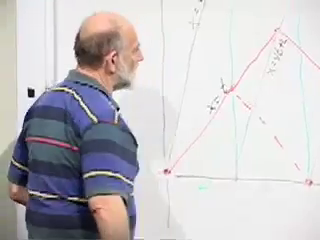
\includegraphics[width=0.72\textwidth]{lecture_01_figure_04.png}\caption{El rayo de luz hacia delante \(x=t\) que se encuentra con la línea de universo central móvil.}\lectureframe{01:02:33}\end{figure}

La geometría completa puede dibujarse sin que una persona de pie obstaculice la pizarra:

\begin{figure}[H]\centering
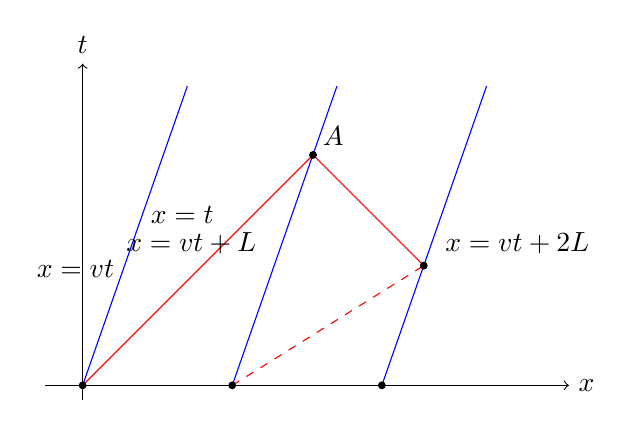
\begin{tikzpicture}[scale=0.95]
\draw[->] (-0.5,0) -- (6.5,0) node[right] {$x$};
\draw[->] (0,-0.2) -- (0,4.3) node[above] {$t$};
\draw[blue] (0,0) -- (1.4,4.0);
\draw[blue] (2.0,0) -- (3.4,4.0);
\draw[blue] (4.0,0) -- (5.4,4.0);
\draw[red] (0,0) -- (3.08,3.08);
\draw[red] (3.08,3.08) -- (4.56,1.60);
\draw[red,dashed] (2.0,0) -- (4.56,1.60);
\fill (0,0) circle (1.5pt);
\fill (2.0,0) circle (1.5pt);
\fill (4.0,0) circle (1.5pt);
\fill (3.08,3.08) circle (1.5pt);
\fill (4.56,1.60) circle (1.5pt);
\node[left] at (0.55,1.55) {$x=vt$};
\node[left] at (2.45,1.9) {$x=vt+L$};
\node[right] at (4.72,1.9) {$x=vt+2L$};
\node[left] at (1.88,2.28) {$x=t$};
\node[above right] at (3.08,3.08) {$A$};
\end{tikzpicture}\caption{Las señales luminosas determinan la línea de simultaneidad del sistema móvil.}\end{figure}

Enviemos desde el origen un rayo de luz hacia la derecha. Sea \(A\) la intersección con la línea de universo central. Las dos ecuaciones en \(A\) son
\begin{align}
x&=t,\\
x&=vt+L.
\end{align}
Al sustituir, obtenemos
\begin{equation}
t=vt+L,
\end{equation}
y, por tanto,
\begin{equation}
t_A=x_A=\frac{L}{1-v}.
\label{eq:point-a}
\end{equation}

Desde \(A\), tracemos hacia atrás un rayo de luz que se desplaza hacia la izquierda hasta la línea de universo móvil de la derecha. Su ecuación tiene la forma
\begin{equation}
x+t=b.
\end{equation}
Como pasa por \(A\), la ecuación~\eqref{eq:point-a} determina la constante:
\begin{equation}
b=x_A+t_A=\frac{2L}{1-v}.
\end{equation}
Así pues, el rayo hacia atrás satisface
\begin{equation}
x+t=\frac{2L}{1-v}.
\label{eq:backward-ray}
\end{equation}

La intersección con la línea de universo de la derecha se obtiene de
\begin{align}
x+t&=\frac{2L}{1-v},\\
x&=vt+2L.
\end{align}
Al eliminar \(x\),
\begin{align}
(1+v)t
  &=2L\left(\frac{1}{1-v}-1\right)\\
  &=\frac{2Lv}{1-v},
\end{align}
por lo que
\begin{equation}
t=\frac{2Lv}{1-v^2}.
\end{equation}
Al sustituir en \(x=vt+2L\), se obtiene
\begin{equation}
x=\frac{2L}{1-v^2}.
\end{equation}
Las coordenadas mismas importan menos que su cociente:
\begin{equation}
\frac{t}{x}=v.
\end{equation}
Por tanto, todos los sucesos simultáneos con el origen según los relojes móviles están en
\begin{equation}
t=vx,
\label{eq:simultaneity-c-one}
\end{equation}
mientras que el origen móvil sigue la trayectoria
\begin{equation}
x=vt.
\label{eq:moving-time-axis}
\end{equation}
Los dos ejes están inclinados simétricamente alrededor del rayo de luz a \(45^\circ\).

Todos los puntos de \(x=vt\) tienen la misma posición primada, \(x'=0\), mientras que sus tiempos primados varían. Todos los puntos de \(t=vx\) tienen el mismo tiempo primado, \(t'=0\), mientras que sus posiciones primadas varían. Por tanto, una línea es el eje temporal primado y la otra, el eje espacial primado. La larga construcción con señales era necesaria para determinar la segunda línea; no podía deducirse solo de la línea de universo móvil.

Para restablecer las unidades ordinarias en la ecuación~\eqref{eq:simultaneity-c-one}, hace falta
\begin{equation}
t=\frac{v}{c^2}x.
\label{eq:simultaneity-dimensional}
\end{equation}
El factor \(c^2\) explica por qué la imagen newtoniana funciona tan bien en la vida cotidiana. Para velocidades muy pequeñas en comparación con \(c\), la pendiente de la línea de simultaneidad móvil es ínfima.

\begin{figure}[H]\centering
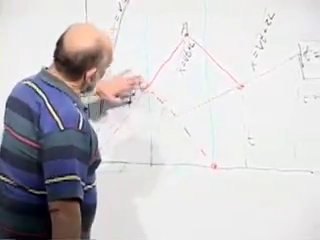
\includegraphics[width=0.72\textwidth]{lecture_01_figure_05.png}\caption{Con \(c=1\), los ejes primados temporal y de simultaneidad son simétricos respecto del rayo de luz.}\lectureframe{01:15:40}\end{figure}

\begin{figure}[H]\centering
\begin{tikzpicture}[scale=1.0]
\draw[->] (-2.2,0) -- (5.2,0) node[right] {$x$};
\draw[->] (0,-0.2) -- (0,4.9) node[above] {$t$};
\draw[red] (0,0) -- (3.9,3.9);
\draw[red] (0,0) -- (-1.8,1.8);
\draw[blue] (0,0) -- (1.8,4.5);
\draw[blue,dashed] (0,0) -- (4.5,1.8);
\node[right] at (3.9,3.9) {$x=t$};
\node[left] at (-1.8,1.8) {$x=-t$};
\node[above] at (1.8,4.5) {$x'=0$};
\node[right] at (4.5,1.8) {$t'=0$};
\end{tikzpicture}\caption{Los ejes primados y los rayos de luz invariantes en unidades \(c=1\).}\end{figure}

\section{Derivación de la transformación de Lorentz}

La geometría determina dónde se anula cada coordenada primada. Sobre el eje temporal móvil \(x=vt\), debe cumplirse \(x'=0\). Sobre el eje de simultaneidad móvil \(t=vx\), debe cumplirse \(t'=0\). Las relaciones lineales más generales que tienen esos conjuntos de ceros pueden escribirse así:
\begin{align}
x'&=\frac{x-vt}{F(v)},\\
t'&=\frac{t-vx}{G(v)}.
\label{eq:fg-ansatz}
\end{align}
Los factores \(F\) y \(G\) permiten que las escalas de las coordenadas primadas difieran de las galileanas, aunque ya hayamos determinado la ubicación de los ejes. La linealidad se desprende de la homogeneidad del espacio y el tiempo: trasladar un experimento no puede cambiar la ley de transformación.\editorialnote{Este breve argumento de linealidad hace explícita una hipótesis usada implícitamente en la derivación en la pizarra.}

En este punto, la geometría ya nos ha dicho mucho, pero no todo. Los numeradores fijan la inclinación de los ejes. No fijan la separación entre unidades a lo largo de ellos. Esa información de escala que aún falta es precisamente lo que representan \(F(v)\) y \(G(v)\).

Impongamos ahora que la velocidad de la luz sea invariante. Un rayo que se desplaza hacia la derecha y satisface \(x=t\) también debe satisfacer \(x'=t'\). A lo largo de ese rayo,
\begin{align}
x'&=\frac{(1-v)t}{F(v)},\\
t'&=\frac{(1-v)t}{G(v)}.
\end{align}
La igualdad para todos los puntos del rayo exige
\begin{equation}
F(v)=G(v).
\end{equation}
Por tanto, podemos escribir
\begin{align}
x'&=\frac{x-vt}{F(v)},\\
t'&=\frac{t-vx}{F(v)}.
\label{eq:common-f}
\end{align}

Este paso introduce en el álgebra la primera exigencia genuinamente einsteiniana. La misma línea geométrica es un rayo de luz para ambos observadores, así que las dos coordenadas primadas deben aumentar por igual a lo largo de ella cuando \(c=1\). Si los factores de las dos ecuaciones fueran distintos, la velocidad primada diferiría de la unidad.

Queda una función desconocida. Multipliquemos la ecuación~\eqref{eq:common-f} por \(F(v)\):
\begin{align}
F(v)x'&=x-vt,\\
F(v)t'&=t-vx.
\end{align}
Multiplicando la segunda ecuación por \(v\) y sumándola a la primera, eliminamos \(t\) y obtenemos
\begin{equation}
(1-v^2)x=F(v)(x'+vt').
\end{equation}
De manera análoga,
\begin{equation}
(1-v^2)t=F(v)(t'+vx').
\end{equation}
Por tanto, la transformación inversa es
\begin{align}
x&=\frac{F(v)}{1-v^2}(x'+vt'),\\
t&=\frac{F(v)}{1-v^2}(t'+vx').
\end{align}

El principio de relatividad hace recíprocos los dos sistemas. Si la estación ve que el tren se mueve a \(+v\), el tren ve que la estación se mueve a \(-v\). Por consiguiente, las ecuaciones inversas deben tener la misma forma que las directas, pero con el signo de \(v\) invertido. Sus factores prefactores deben satisfacer
\begin{equation}
\frac{F(v)}{1-v^2}=\frac{1}{F(v)}.
\end{equation}
Por tanto,
\begin{equation}
F(v)^2=1-v^2,
\end{equation}
y la continuidad con la transformación identidad en \(v=0\) selecciona la raíz positiva:
\begin{equation}
F(v)=\sqrt{1-v^2}.
\end{equation}

El resultado no se ha ajustado a ningún pulso luminoso particular. Se desprende de los ejes determinados por la sincronización, de que la velocidad de la luz es común y de la exigencia de que ninguno de los sistemas inerciales tenga un lugar privilegiado.

La transformación de Lorentz en unidades con \(c=1\) es
\begin{align}
x'&=\frac{x-vt}{\sqrt{1-v^2}},\\
t'&=\frac{t-vx}{\sqrt{1-v^2}}.
\label{eq:lorentz-c-one}
\end{align}
Su inversa es
\begin{align}
x&=\frac{x'+vt'}{\sqrt{1-v^2}},\\
t&=\frac{t'+vx'}{\sqrt{1-v^2}}.
\end{align}

\begin{figure}[H]\centering
\includegraphics[width=0.76\textwidth]{lecture_01_figure_06.png}\caption{La transformación de Lorentz \(c=1\) completa en la pizarra.}\lectureframe{01:32:38}\end{figure}

La novedad esencial ya se aprecia en la ecuación del tiempo. El tiempo no se traslada sin cambios de un sistema a otro. Una coordenada temporal primada combina tiempo y posición no primados. Por consiguiente, \(t=\text{constant}\) y \(t'=\text{constant}\) describen conjuntos distintos de sucesos.

El término de mezcla no es una corrección opcional añadida a posteriori. Sin él, la línea \(t'=0\) seguiría siendo horizontal, la simultaneidad distante continuaría siendo universal y la transformación no podría conservar la velocidad de la luz.

\section{Restablecer la velocidad de la luz y comprobar el resultado}

Cuando \(c\ne1\), la coherencia dimensional restituye los factores que faltaban. La razón \(v^2/c^2\) es adimensional, mientras que \((v/c^2)x\) tiene unidades de tiempo. Así pues,
\begin{align}
x'&=\frac{x-vt}{\sqrt{1-v^2/c^2}},\\
t'&=\frac{t-(v/c^2)x}{\sqrt{1-v^2/c^2}}.
\label{eq:lorentz-dimensional}
\end{align}
La transformación inversa se obtiene invirtiendo el signo de \(v\):
\begin{align}
x&=\frac{x'+vt'}{\sqrt{1-v^2/c^2}},\\
t&=\frac{t'+(v/c^2)x'}{\sqrt{1-v^2/c^2}}.
\end{align}
Si introducimos
\begin{equation}
\gamma=\frac{1}{\sqrt{1-v^2/c^2}}
\end{equation}
obtenemos la forma compacta habitual, pero escribir el denominador explícitamente permite seguir la derivación.

Numéricamente, \(c\simeq3\times10^8\,\mathrm{m/s}\), por lo que \(c^2\simeq9\times10^{16}\,\mathrm{m^2/s^2}\). El denominador grande hace que, en la mayoría de los experimentos mecánicos, la inclinación de la simultaneidad y el factor \(v^2/c^2\) sean imperceptibles. Que sean pequeños explica el éxito de Galileo; no restablece el tiempo absoluto.

\begin{figure}[H]\centering
\includegraphics[width=0.76\textwidth]{lecture_01_figure_07.png}\caption{La transformación de Lorentz tras restablecer los factores de \(c\).}\lectureframe{01:35:58}\end{figure}

Dos comprobaciones son inmediatas. Primero, consideremos \(v\ll c\). Entonces \(v^2/c^2\) es despreciable y, para distancias ordinarias, el término de relatividad de la simultaneidad \(vx/c^2\) también lo es. La ecuación~\eqref{eq:lorentz-dimensional} se reduce a
\begin{equation}
t'\approx t,\qquad x'\approx x-vt.
\end{equation}
Se recupera la relatividad galileana como aproximación a bajas velocidades.

Segundo, comprobemos el caso de un rayo de luz. Una vez restituido \(c\), un rayo que se propaga hacia la derecha satisface \(x=ct\), no \(x=t\). Al sustituir, se obtiene
\begin{align}
x'&=\frac{(c-v)t}{\sqrt{1-v^2/c^2}},\\
t'&=\frac{(1-v/c)t}{\sqrt{1-v^2/c^2}}.
\end{align}
Como \(c-v=c(1-v/c)\),
\begin{equation}
x'=ct'.
\end{equation}
El observador primado mide la misma velocidad \(c\). Para un rayo que se propaga hacia la izquierda, al sustituir \(x=-ct\) se obtiene, de manera análoga,
\begin{equation}
x'=-ct'.
\end{equation}
La transformación describe correctamente la luz que se propaga en cualquiera de las dos direcciones.

La distinción entre \(x=t\) y \(x=ct\) ofrece una comprobación dimensional instructiva. La primera expresión solo es correcta en unidades en las que \(c=1\). Restituir unidades ordinarias en la transformación y dejar la ecuación del rayo en unidades naturales mezclaría dos convenciones y daría un resultado erróneo. La coherencia dimensional permite detectar el error de inmediato.

\section{El criterio del punto medio}

\begin{classroomqa}
\audiencequestion{Supongamos que un observador recibe dos destellos en el mismo instante, pero no está a mitad de camino entre sus fuentes. ¿Puede concluir que los destellos se emitieron simultáneamente?
\lecturetimestamp{01:42:55}}
\lecturerresponse{No. Que los tiempos de llegada sean iguales implica que los tiempos de emisión también lo son únicamente para el observador situado espacialmente a mitad de camino entre las dos fuentes en el marco pertinente. Un receptor más cerca de una fuente puede recibir ambos destellos a la vez aunque el destello más lejano se haya emitido antes. En la construcción móvil, la línea de universo del punto medio \(x=vt+L\) es, por tanto, esencial. Se sigue el rayo que avanza \(x=t\) hasta que alcanza ese punto medio; luego se traza un rayo de luz hacia atrás hasta \(x=vt+2L\). Según el marco móvil, ese segundo suceso extremo es simultáneo con el origen; un suceso cualquiera de llegada simultánea en otro lugar no lo es.}
\end{classroomqa}

Hemos llegado a la transformación completa de coordenadas, pero todavía no a sus consecuencias más conocidas. A continuación veremos la contracción de la longitud, la dilatación del tiempo y el tiempo propio, y después el momento y la energía relativistas. Los fundamentos ya están establecidos: cada marco inercial puede emplear las mismas leyes y medir la misma velocidad de la luz solo porque el espacio y el tiempo se mezclan, y porque la simultaneidad a distancia depende del marco y no es absoluta.